\documentclass[14pt, a4paper]{extarticle}
\usepackage{GOST}
\usepackage{array}
\usepackage{verbatim}
\usepackage[detect-all]{siunitx}
\usepackage{amsmath}
\usepackage{amssymb}
\usepackage[utf8]{inputenc}
\usepackage{hyperref}

\usepackage{ifthen}


\usepackage{tempora}



\makeatletter
\renewcommand\@biblabel[1]{#1.}
\makeatother

% Для листинга кода:
\usepackage{listings}
\lstset{ %
	language=c++,                 % выбор языка для подсветки (здесь это С)
	basicstyle=\small\sffamily, % размер и начертание шрифта для подсветки кода
	numbers=left,               % где поставить нумерацию строк (слева\справа)
	numberstyle=\tiny,           % размер шрифта для номеров строк
	stepnumber=1,                   % размер шага между двумя номерами строк
	numbersep=5pt,                % как далеко отстоят номера строк от подсвечиваемого кода
	showspaces=false,            % показывать или нет пробелы специальными отступами
	showstringspaces=false,      % показывать или нет пробелы в строках
	showtabs=false,             % показывать или нет табуляцию в строках
	frame=single,              % рисовать рамку вокруг кода
	tabsize=2,                 % размер табуляции по умолчанию равен 2 пробелам
	captionpos=t,              % позиция заголовка вверху [t] или внизу [b] 
	breaklines=true,           % автоматически переносить строки (да\нет)
	breakatwhitespace=false, % переносить строки только если есть пробел
	escapeinside={\#*}{*)}   % если нужно добавить комментарии в коде
}


%для графиков
\usepackage{pgfplots}
\usepackage{filecontents}
\usetikzlibrary{datavisualization}
\usetikzlibrary{datavisualization.formats.functions}

\begin{document}
	
	\begin{table}[ht]
		\centering
		\begin{tabular}{|c|p{400pt}|} 
			\hline
			\begin{tabular}[c]{@{}c@{}} 
\includegraphics[scale=1]{source/baum.jpg} \\\end{tabular} &
			\footnotesize\begin{tabular}[c]{@{}c@{}}\textbf{Министерство~науки~и~высшего~образования~Российской~Федерации}\\\textbf{Федеральное~государственное~бюджетное~образовательное~учреждение}\\\textbf{~высшего~образования}\\\textbf{«Московский~государственный~технический~университет}\\\textbf{имени~Н.Э.~Баумана}\\\textbf{(национальный~исследовательский~университет)»}\\\textbf{(МГТУ~им.~Н.Э.~Баумана)}\\\end{tabular}  \\
			\hline
		\end{tabular}
	\end{table}
	\noindent\rule{\textwidth}{4pt}
	\noindent\rule[14pt]{\textwidth}{1pt}
	\hfill 
	\noindent
	\makebox{ФАКУЛЬТЕТ~}%
	\makebox[\textwidth][l]{\underline{~«Информатика и системы управления»~~~~~~~~~~~~~~~~~~~~~~~~~~~~~~~~~}}%
	\\
	\noindent
	\makebox{КАФЕДРА~}%
	\makebox[\textwidth][l]{\underline{~«Программное обеспечение ЭВМ и информационные технологии»~}}%
	\\
	
	\begin{center}
		\vspace{1.5cm}
		{\bf\huge Отчёт\par}
		{\bf\Large по лабораторной работе № 6\par}
		\vspace{0.7cm}
	\end{center}
	
	
	\noindent
	\makebox{\large{\bf Название:}~~~}
	\makebox[\textwidth][l]{\large\underline{Реализация монитора Хоара «Читатели-писатели»~~~~~~}}\\
	
	\noindent
	\makebox{\large{\bf Дисциплина:}~~~}
	\makebox[\textwidth][l]{\large\underline{~Операционные системы~~~~~~~~~~~~~~~~~~~~~~~~~~}}\\
	
	\vspace{1.5cm}
	\noindent
	\begin{tabular}{l c c c c c}
		Студент      & ~ИУ7-55Б~               & \hspace{2.5cm} & \hspace{2cm}                 & &  Д.В. 
		Сусликов \\\cline{2-2}\cline{4-4} \cline{6-6} 
		\hspace{3cm} & {\footnotesize(Группа)} &                & {\footnotesize(Подпись, дата)} & & {\footnotesize(И.О. Фамилия)}
	\end{tabular}
	
	\noindent
	\begin{tabular}{l c c c c}
		Преподаватель & \hspace{5cm}   & \hspace{2cm}                 & & ~~~~~~Н.Ю. Рязанова~~~~~~\\\cline{3-3} \cline{5-5} 
		\hspace{3cm}  &                & {\footnotesize(Подпись, дата)} & & {\footnotesize(И.О. Фамилия)}
	\end{tabular}
	
	\vspace{0.6cm}
	\begin{center}	
		\vfill
		\large \textit {Москва, 2020}
	\end{center}
	
	\thispagestyle {empty}
	\pagebreak
	
	% СОДЕРЖАНИЕ 
	\clearpage
	\tableofcontents
	
	
	% ВВЕДЕНИЕ
	\clearpage
	\section*{Задание}
	\addcontentsline{toc}{section}{Задание}
	В лабораторной работе необходимо разработать многопоточное приложение, используя API ОС Windows такие как, потоки, события (event) и мьютексы (mutex). Потоки разделяют единственную глобальную переменную. Приложение реализует монитор Хоара «Читатели-писатели».\par
	
	
	\section*{Программа}
	\addcontentsline{toc}{section}{Программа}
	В Листинге 1 описан код программы.\newline
	\begin{lstlisting}[caption= Задание]
	#include <stdio.h>
	#include <windows.h>
	#include <iostream>
	
	#define OK 0
	#define ERROR 1
	
	#define WRITERS 3
	#define READERS 5
	#define ITERS 5
	
	int value = 0;
	
	HANDLE writers[WRITERS];
	HANDLE readers[READERS];
	
	HANDLE can_read;
	HANDLE can_write;
	HANDLE mutex;
	
	bool is_active_writer = false;
	unsigned int active_readers = 0;
	
	unsigned int waiting_writers = 0;
	unsigned int waiting_readers = 0;
	
	void start_write()
	{
		InterlockedIncrement(&waiting_writers);
		if (is_active_writer || active_readers > 0)
			WaitForSingleObject(can_write, INFINITE);
		
		InterlockedDecrement(&waiting_writers);
		is_active_writer = true;
		ResetEvent(can_write);
	}
	
	void stop_write()
	{
		is_active_writer = false;
		if (waiting_writers)
			SetEvent(can_write);
		else
			SetEvent(can_read);
	}
	
	void start_read()
	{
		InterlockedIncrement(&waiting_readers);
		if (is_active_writer || waiting_writers > 0)
			WaitForSingleObject(can_read, INFINITE);
		
		WaitForSingleObject(mutex, INFINITE);
		
		InterlockedDecrement(&waiting_readers);
		InterlockedIncrement(&active_readers);
		SetEvent(can_read);
		
		ReleaseMutex(mutex);
	}
	
	void stop_read()
	{
		InterlockedDecrement(&active_readers);
		if (active_readers == 0)
			SetEvent(can_write);
	}
	
	DWORD WINAPI reader(LPVOID lpParam)
	{
		while (value < WRITERS * ITERS)
		{
			start_read();
			printf("Reader %d with id %d read %d\n", (int)lpParam, GetCurrentThreadId(), value);
			stop_read();
			Sleep(200);
		}
		return OK;
	}
	
	DWORD WINAPI writer(LPVOID lpParam)
	{
		for (int i = 0; i < ITERS; i++)
		{
			start_write();
			value++;
			printf("Writer %d with id %d wrote %d\n", (int)lpParam, GetCurrentThreadId(), value);
			stop_write();
			Sleep(200);
		}
		return OK;
	}
	
	bool check_error(HANDLE cur, const char* msg)
	{
		if (cur == NULL)
		{
			CloseHandle(mutex);
			CloseHandle(can_read);
			CloseHandle(can_write);
			perror(msg);
			return false;
		}
		return true;
	}
	
	int main()
	{
		mutex = CreateMutex(NULL, FALSE, NULL);
		if (mutex == NULL)
		{
			perror("mutex");
			return ERROR;
		}
		
		can_read = CreateEvent(NULL, FALSE, FALSE, TEXT("ReadEvent"));
		if (can_read == NULL)
		{
			CloseHandle(mutex);
			perror("can_read");
			return ERROR;
		}
		
		can_write = CreateEvent(NULL, TRUE, FALSE, TEXT("WriteEvent"));
		if (can_write == NULL)
		{
			CloseHandle(mutex);
			CloseHandle(can_read);
			perror("can_write");
			return ERROR;
		}
		
		for (int i = 0; i < WRITERS; i++)
		{
			writers[i] = CreateThread(NULL, 0, &writer, (LPVOID)i, 0, NULL);
			if (!check_error(writers[i], "Thread"))
				return ERROR;
		}
		
		for (int i = 0; i < READERS; i++)
		{
			readers[i] = CreateThread(NULL, 0, &reader, (LPVOID)i, 0, NULL);
			if (!check_error(readers[i], "Thread"))
				return ERROR;
		}
		
		WaitForMultipleObjects(WRITERS, writers, TRUE, INFINITE);
		WaitForMultipleObjects(READERS, readers, TRUE, INFINITE);
		
		CloseHandle(mutex);
		CloseHandle(can_read);
		CloseHandle(can_write);
		
		return 0;
	}
	\end{lstlisting}
	
	\newpage
	Ниже на Рисунке 1 показан пример работы данной программы.
	\begin{figure}[h!]
		\centering{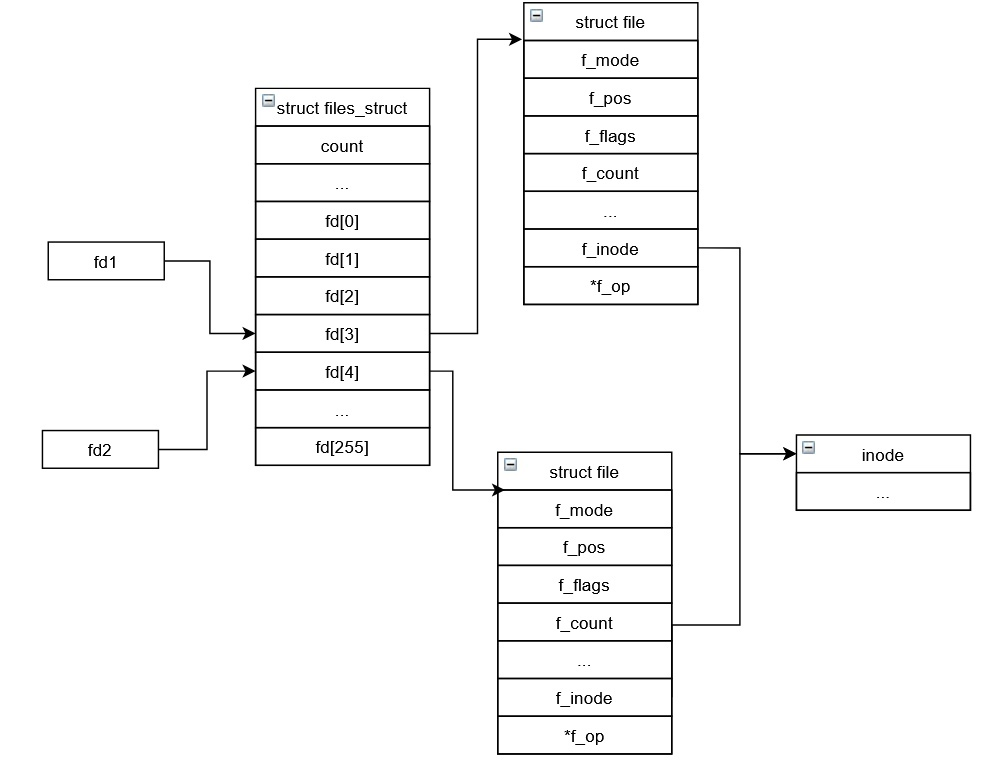
\includegraphics[scale=1]{source/2.jpg}}
		\caption{Пример работы программы}
	\end{figure}
	\newpage

\end{document}